\documentclass{beamer}


% Load essential packages
\usepackage{hyperref} % Only load once to avoid conflicts
\usepackage{stile}
\usepackage{subcaption}
\usepackage{tcolorbox}
\usepackage[font=scriptsize,skip=1pt]{caption}
\usepackage[T1]{fontenc}
\usepackage{csquotes}
\usepackage[backend=biber, style=authoryear, maxnames=3, minnames=1, abbreviate=false, date=long, url=false, isbn=false, doi=false]{biblatex}
\addbibresource{lecture2/bib.bib} % Ensure this matches your bibliography file name

\interfootnotelinepenalty=10000

\usepackage{latexsym, amsmath, xcolor, multicol, booktabs, calligra}
\usepackage{graphicx, pstricks, listings, stackengine}

% Hyperref setup
\hypersetup{
    hidelinks,
    colorlinks=true,
    linkcolor=black,
    citecolor=deepblue,
    urlcolor=black
}

% Font theme for Beamer
\usefonttheme[onlymath]{serif}

% Custom definitions
\def\cmd#1{\texttt{\color{red}\footnotesize $\backslash$#1}}
\def\env#1{\texttt{\color{blue}\footnotesize #1}}
\definecolor{deepblue}{rgb}{0,0,0.5}
\definecolor{deepred}{rgb}{0.6,0,0}
\definecolor{deepgreen}{rgb}{0,0.5,0}
\definecolor{halfgray}{gray}{0.55}

% Beamer color settings
\setbeamercolor{block title}{bg=blue!70!white, fg=white}
\setbeamercolor{block body}{bg=blue!10!halfgray, fg=white}
\setbeamercolor{section in head/foot}{fg=white}
\setbeamercolor{subsection in head/foot}{fg=white}
\setbeamercolor{title in head/foot}{fg=white}


% Listings settings for code highlighting
\lstset{
    basicstyle=\ttfamily\small,
    keywordstyle=\bfseries\color{deepblue},
    emphstyle=\ttfamily\color{deepred},
    stringstyle=\color{deepgreen},
    numbers=left,
    numberstyle=\small\color{halfgray},
    rulesepcolor=\color{red!20!green!20!blue!20},
    frame=shadowbox,
}

\author{Freya Rubel}
\title{Trade, Migration and Global Challenges}
\subtitle{Gains from Trade}
\institute{}
\date{27.10.2026}

\graphicspath{{lecture2/}}

\begin{document}

\begin{frame}
    \titlepage
\end{frame}

\begin{frame}
    \tableofcontents[sectionstyle=show, subsectionstyle=show/shaded/hide, subsubsectionstyle=show/shaded/hide]
\end{frame}

\section{Definition}
\begin{frame}{What is a Gain?}
\begin{itemize} 
    \item Advantages that trading countries enjoy through the specialization and division of labour compared to a state of autarky.
    \item As soon as the utility of an average/representative citizen increases from international trade, trade is considered \textbf{welfare increasing}. 
\end{itemize}
\end{frame}

 \begin{frame}{Static vs. Dynamic Gain}
\textbf{Static gains:} What a country can gain through the reallocation of factors into sectors where that country is producing most efficiently. They appear immediately through a more efficient allocation of factors. \vspace{0.1cm}\\ \pause
\textbf{Dynamic gains:} Dynamic gains develop over time. They can appear through clusters of skilled labour force, R\&D institutions, and increased technological progress.  
\end{frame}

\begin{frame}[t]{Product Variety}
\begin{itemize}
    \item Standard economic theory assumes that economic agents have convex indifference functions $\rightarrow$ Consumers love variety 
    % few people always prefer chocolate over pasta. We don't want to live in a country that only offers us chocolate or one that only offers us pasta. But those goods are at present produced in very different regions of the world. The fact that we get to enjoy both is due to international trade, and it lifts us onto a higher indifference curve
\end{itemize}
\end{frame}


\begin{frame}[t]{Product Variety}
\begin{itemize}
    \item Standard economic theory assumes that economic agents have convex indifference functions $\rightarrow$ Consumers love variety 
\end{itemize}
\begin{figure}
    \centering
    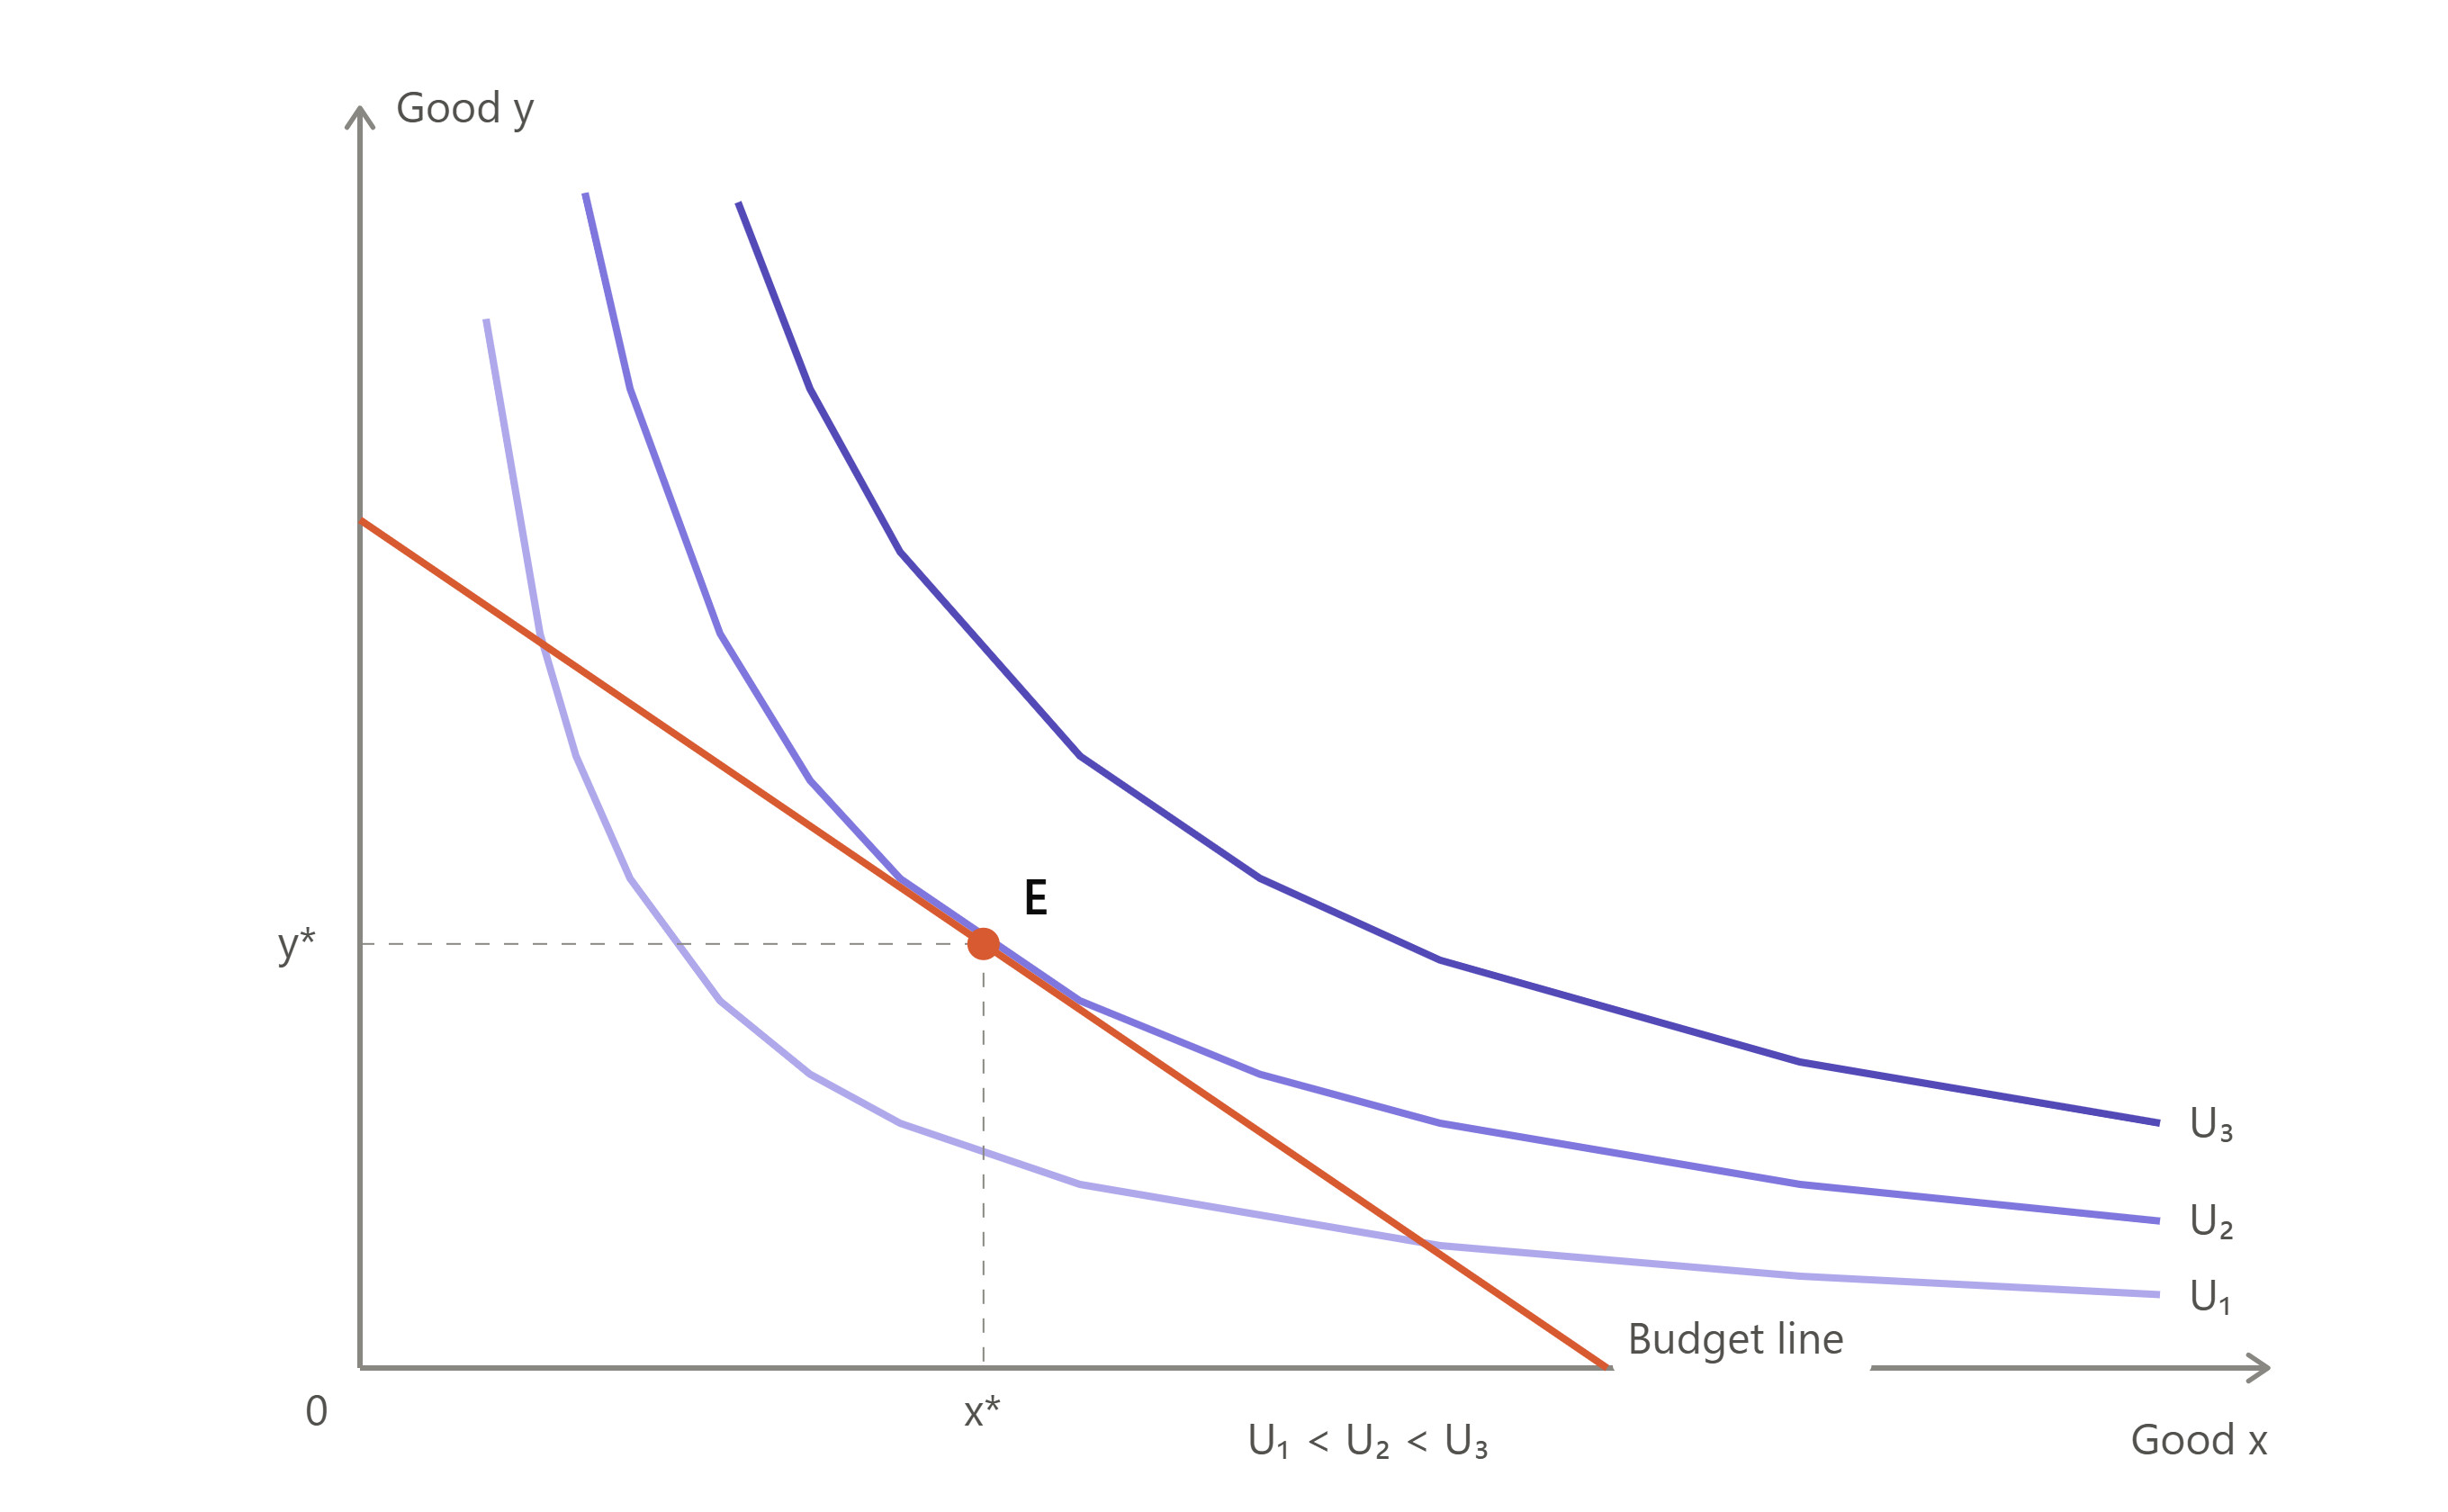
\includegraphics[width=0.8\linewidth]{lecture2/convex_indifference_curves_budget_tangency.png}
\end{figure}
    
\end{frame}

\section{Comparative Advantage - Theoretical Model}
\begin{frame}{Standard Assumptions}
\textbf{Theory of International Trade}
\begin{itemize} \small
    \item Factor markets are domestic % I talked about factors briefly last week. A Factor in economic is sort of a resource that is used for production. Those can be labor, raw materials, 
    \item Goods (and services) markets are international
\end{itemize}
Goods (and services) enter a consumer's utility function directly and can be freely traded across international borders. \\
Factors affect the utility of consumers through the income they generate; their endowment is fixed domestically, and they cannot be traded at all. 
% \textcolor{gray}{\scriptsize While this might seem like a very strong assumption given factor mobility, it can be made plausibly when we consider anything a good as soon as it can be traded.} 
\end{frame}

\begin{frame}{Standard Assumptions Cont.}
 Standardized models in neoclassical trade theory also assume that:
 \begin{itemize} \small
     \item All consumers in a given country have identical homothetic preferences (representative agent)
     \begin{itemize} \scriptsize
         \item Homothetic preferences: ratios of goods demanded by consumers will depend only on relative prices, not on income.
         % we just looked at the utility that you get from variety. Consumers like a variety and prefer a certain ratio of the two goods. In our standardized model, this ratio is not changing no matter their income. In reality, this is not true. Can you come up with an example of two goods where your income determins the ratio in which you prefer to consume them? Bread and Vacation trips -> with increasing income, the ratio of bread compared to vacation trips changes. The ratio will shift towards the vacation trips away from bread. However, we are not considering such cases. It illustrates how those assumptions underlying economic models are oftentimes not realistic. 
     \end{itemize}
     \item There are no long-term adjustments (static model)
     \item Perfect competition in production and consumption (price equals marginal costs of production)
     \begin{itemize} \scriptsize
         \item Every economic agent takes the prices as given and believes that their impact on the market is negligable
     \end{itemize}
     \item All economic agents make the perfect rational choices that maximize their utility % they have perfect information about the goods that are traded on the market, they know beforehand, how happy this bar of soap from France will make them. There are no bad surprises. We have komplete knowledge 
     \item Constant returns to scale % we talked about this last week. While in reality we know that increased quantity in production is decreasing the cost per unit produced, economic theory assumes that this does not exist because otherwise, it should lead to a lot of natural monopolies. It is considered a market failure that calls for state intervention 
     \item No distortions (no externalities, no taxes/subsidies, no tariffs or any other form of government intervention)
     % do you know what is meant by externalities? There are positive as well as negative externalities
     % classic example: honey has positive externalities because the bees that produce the honey are also acting as unpaid labour in neighbouring plantations because of the pollination -> this is also called an ecosystem service
     % A classic negative externality is carbon dioxide. It is imposing a cost on the general public but is not entering the private cost function of the producing firm. Therefore, the firm is producing more than what would be the social optimum
 \end{itemize}
\end{frame}


\begin{frame}{Background}
    The theoretical concept of gains from trade based on an article by \textcite{samuelson_comparative_advantage}, who was the first one to formulate the gains from trade. 
    \begin{itemize}
        \item Contribution: under perfect competition, opening up to trade expands the production possibility frontier (PPF) and leads to Pareto superior outcomes. % everyone is better off, no one is worse off
    \end{itemize}
    \textcite{deardorff_1980} later demonstrated the general validity of the concept of the \textit{Comparative Advantage}.
\end{frame}

\begin{frame}{Numeric Example - Setup}
    Both England and Portugal can produce wine and cake. \vspace{0.1cm}\\
    \textbf{England} 
    \begin{itemize} \small
        \item One worker is able to produce 10 cakes \textbf{or} 5 bottles of wine per day.
        \item To produce one bottle of wine, England is foregoing producing how many cakes? \pause \underline{2 cakes} \pause
        \item To produce one cake, England is foregoing producing how many bottles of wine? \pause \underline{0.5 bottles of wine} \pause
    \end{itemize}
    \textbf{Portugal}
    \begin{itemize} \small
        \item One worker is able to produce 5 cakes \textbf{or} 10 bottles of wine per day. 
        \item To produce one bottle of wine, Portugal is foregoing producing how many cakes? \pause \underline{0.5 cakes} \pause
        \item To produce one cake, Portugal is foregoing producing how many bottles of wine? \pause \underline{2 bottles of wine} 
    \end{itemize} % if we think of producing wine and cake as opportunity costs of not producing the alternative good, producing cake is more costly for Portugal than it is for England and producing wine is more costly for England than it is for Portugal. These differences can be historically, geographically and simply due to culture and tradition
\end{frame}

\begin{frame}{Numeric Example - Identify Comparative Advantage}
\textbf{England} has a lower opportunity cost of producing cakes (0.5 bottles of wine per unit of cake) than Portugal (2 bottles of wine per unit of cake). Therefore, England has a \underline{comparative advantage in the production of cake}. \vspace{0.1cm} \\
\textbf{Portugal} has a lower opportunity cost of producing wine (0.5 cakes per bottle of wine) than England (2 cakes per bottle of wine). Therefore, Portugal has a \underline{comparative advantage in the production of wine}.
\end{frame}

\begin{frame}{Numeric Example - Autarky Case}
    Suppose each country has 100 workers that are evenly split between the production of the two goods. \vspace{0.1cm} \\
    The English economy (\begin{small}One worker is able to produce 10 cakes \textbf{or} 5 bottles of wine per day\end{small}) is producing which quantities of which products per day? \pause 
    \begin{itemize} \small
        \item 50 $\times$ 10 cakes = \textbf{500 cakes} \textit{plus} 50 $\times$ 5 bottles of wine = \textbf{250 bottles of wine}. \pause
    \end{itemize}
    The Portuguese economy (\begin{small}One worker is able to produce 5 cakes \textbf{or} 10 bottles of wine per day\end{small}) is producing which quantities of which products per day? \pause 
    \begin{itemize} \small
        \item 50 $\times$ 5 cakes = \textbf{250 cakes} \textit{plus} 50 $\times$ 10 bottles of wine = \textbf{500 bottles of wine}. 
    \end{itemize}
\end{frame}

\begin{frame}{Numeric Example - Specialization}
    Suppose that each country is only producing the good that they have a comparative advantage in. \vspace{0.1cm} \\
    England is specializing in cakes and Portugal is specializing in wine. 
    \begin{itemize}
        \item England is producing 1000 cakes.
        \item Portugal is producing 1000 bottles of wine. 
    \end{itemize}
\end{frame}

\begin{frame}{Numeric Example - Trade}
The exact "price" in terms of bottles of wine for one cake depends on the specific consumer preferences and the bargaining power of the two countries, but it has to be \textbf{in the range between 0.5 bottles of wine and 2 bottles of wine for one cake}. \textcolor{red}{Why?} \pause \\ %If the price falls outside this range, one country won't benefit from trading. If 1 cake costs less than 0.5 bottles of wine: England won't trade. They can produce 1 cake domestically by giving up only 0.5 bottles of wine, so why trade for worse terms? If 1 cake costs more than 2 bottles of wine: Portugal won't trade. They can produce 1 cake domestically by giving up only 2 bottles of wine, so paying more makes no sense.
Suppose that the two countries agree on the following term of trade: \textbf{One bottle of wine for one cake} \vspace{0.15cm}\\
Now, the two countries can trade their produced goods. Suppose that they agree on trading 400 bottles of wine for 400 cakes. \pause % they might do this because the english consumers prefer cake over wine and the portuguese consumers prefer wine over cake
\begin{itemize} \small
    \item England is left with 600 cakes and 400 bottles of wine.
    \item Portugal is left with 400 cakes and 600 bottles of wine.
\end{itemize}
\end{frame}

\begin{frame}{Graphical Explanation}
    \begin{figure}
        \centering
        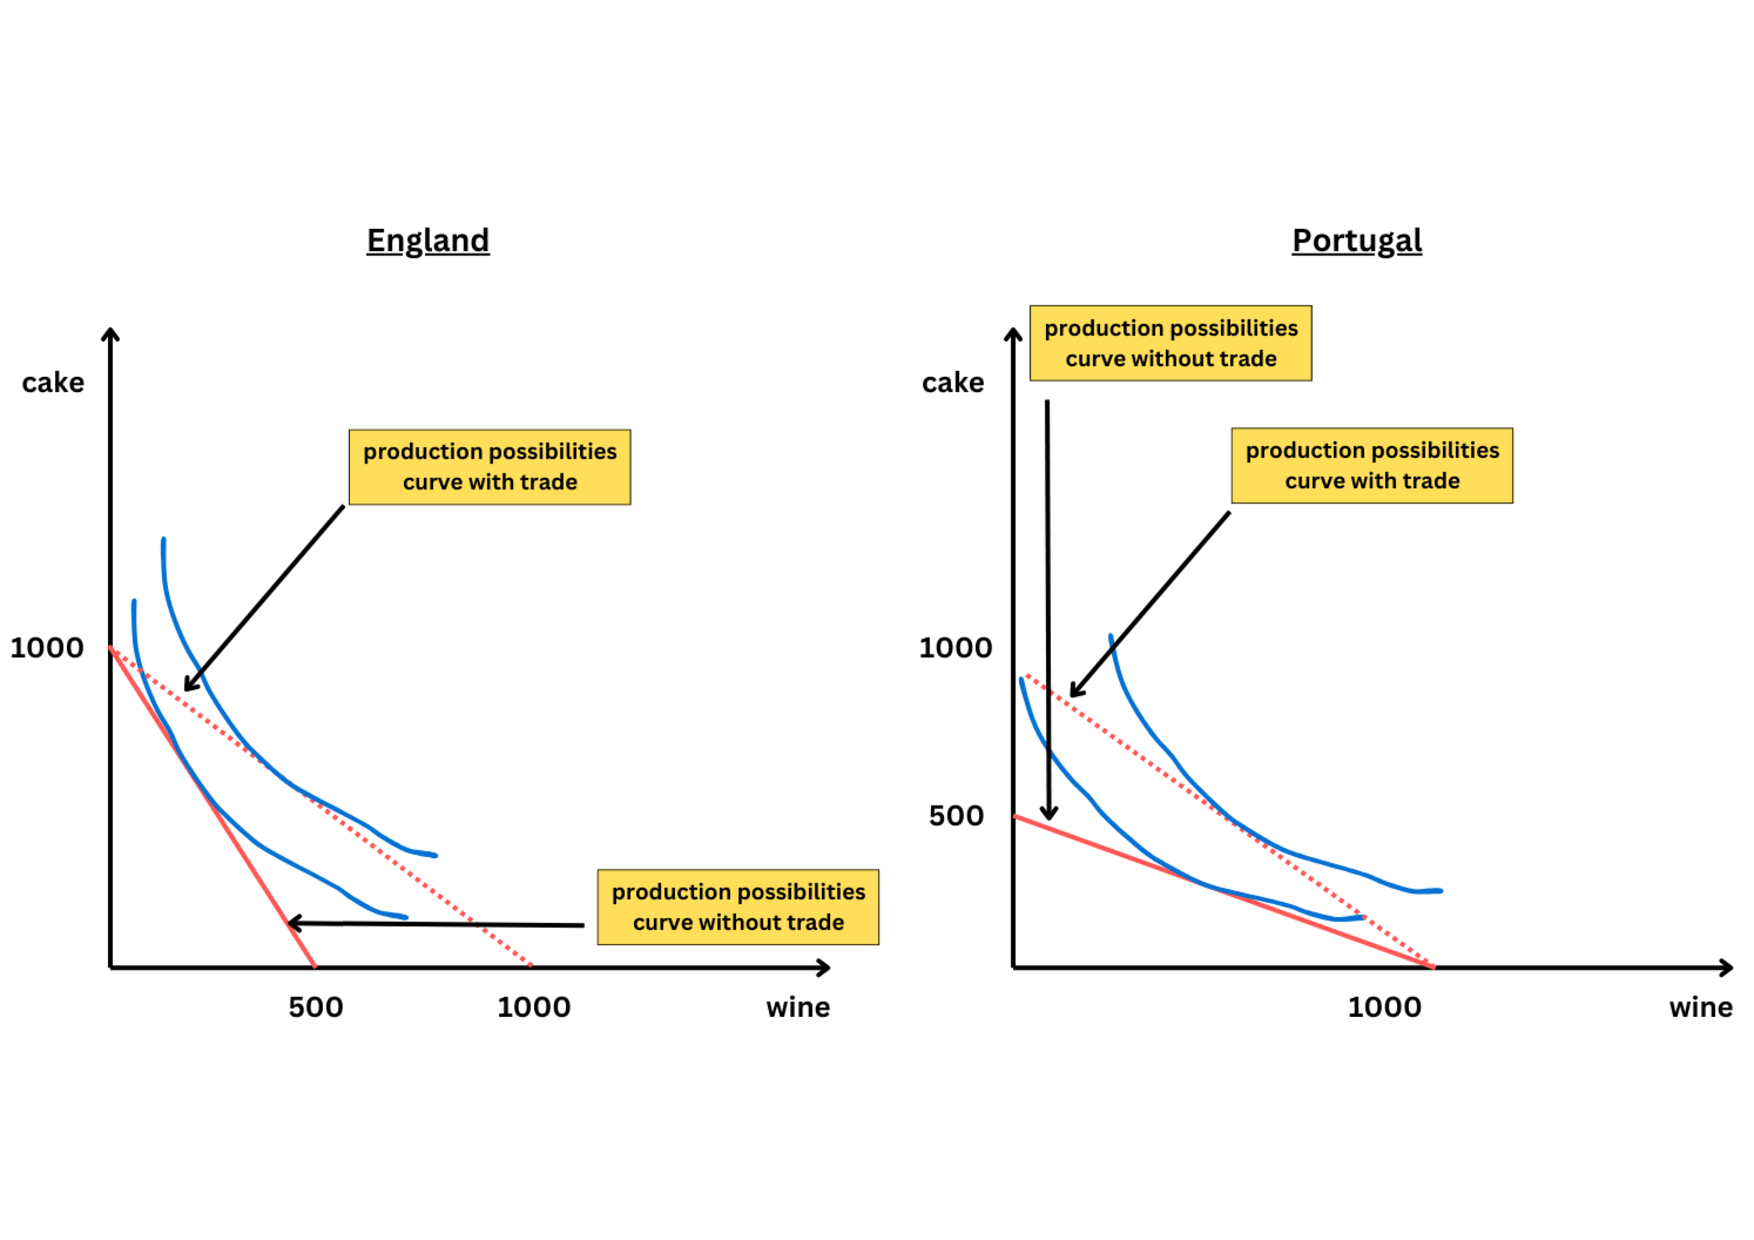
\includegraphics[width=\linewidth]{graphical comparative advantage.pdf}
        \caption{Utility of representative agent in autarky vs. free trade}
    \end{figure}
\end{frame}

\begin{frame}{Differences in Opportunity Costs}
    \textbf{Where do those differences in opportunity costs between countries come from?} \pause
    \begin{itemize} \small
        \item Different endowments (in natural resources)
        \item Climatic factors
        \item Differences in education of the workforce
        \item Differences in history, culture, tradition % there is a learning curve in every task
        \item Technological differences % often result of differences in education and activity of the reserach and development sector
        \item Differences in factor proportions (labor abundant and capital abundant countries)
        \item Differences in infrastructure 
        \item Government policies (subsidies, taxes, and regulation)
    \end{itemize}
\end{frame}

\begin{comment}
\section{Paper on Poverty Alleviation in Vietnam}

\begin{frame}{Paper and Research Question}
    In "\textit{Exporting out of poverty: Provincial poverty in Vietnam and U.S. market access}" \textcite{vietnam_paper} investigates whether a developing country can reduce poverty by gaining increased market access to a large, rich country through trade liberalization. The paper was published in the \textit{Journal of International Economics}. 
    \vspace{0.2cm}\\ % it is one of the first ones to test empirically whether increased market access has a decreasing effect on poverty in developing countries
    \begin{tcolorbox}
         \textcolor{dark}{Research Question:} What was the effect of reduced US tariffs on Vietnamese products on the poverty rate in Vietnam?
    \end{tcolorbox}
   
\end{frame}

\begin{frame}{Background}
    \begin{itemize} \small
        \item Prior to this paper there was little evidence on the effect of bilateral trade agreements (BTA) on poverty
        \item The BTA between the US and Vietnam came into force in 2001
        \begin{itemize}
            \item Tariff drops differed depending on the industry.
            \item U.S. tariffs on Vietnamese products dropped immediately while Vietnamese tariffs on U.S. goods were decreased gradually
        \end{itemize}
        \item From 2001 to 2002, Vietnamese exports to the U.S. grew by 128\%, especially in apparel and clothing accessories
        \item Vietnam's top seven exports to the U.S. are all products that are conventionally classified as being low-skilled labor intensive
        \item Between 2002 and 2004 the national poverty rate in Vietnam fell from 28.9 to 19.5\% $\implies$ But is the BTA the reason for this drop?
    \end{itemize}
\end{frame}

\begin{frame}{Methodology}
\begin{itemize} \small
    \item  \textcite{vietnam_paper} exploits the fact that different provinces in Vietnam were subject to different exposure to the BTA. 
    \item The employment shares for different industries (structure of the economy) varies between the provinces before the BTA come into force.
    \item Given that the tariffs imposed by the U.S. on Vietnamese goods differ depending on the industry, the regional economy on province level faces different tariffs.
    \item He constructs province-level measures of U.S. tariffs based on employment-weighted average industry tariffs using time-invariant pre-BTA employment data.
\end{itemize}
$$\Delta y_{p}=\Delta \theta_t+\beta\Delta \tau_{p}+\Delta \varepsilon_{p}$$
\end{frame}

\begin{frame}{Data}
\begin{itemize} \small
    \item Data on U.S. tariffs stems from the U.S. International Trade Commission's online Tariff Information Center.
    \item The poverty rate (outcome variable) is here defined as the poverty headcount ratio. To calculate this, he uses the Vietnam Household Living Standards Surveys that are representative at the provincial level and provide information on household expenditures, employment, and various other household and individual characteristics.
    \item To calculate the employment shares in different industries on province-level, he uses the 1999 Population and Housing Census made available through Integrated Public Use Microdata Series.
\end{itemize}
\end{frame}

\begin{frame}{Results}
\textcolor{dark}{Primary result:}
    \begin{itemize} \small
        \item All specifications show a positive and statistically significant relationship between provincial poverty and tariffs, indicating that the reduction in U.S. tariffs is associated with differences in poverty reduction across provinces (positive estimate of $\beta$).
        \item The magnitude of the effect is very large in comparison to the overall reduction in poverty in Vietnam between 2002 and 2004.
        \end{itemize}
        \textcolor{dark}{Secondary results:}
        \begin{itemize} \small
        \item Provinces that experienced the greatest reduction in U.S. tariffs received greater inflows of migrants.
        \item For workers with formal low education, the drop in provincial tariffs is associated with faster growth of the mean provincial wage, while for workers with more than a lower secondary education, the impact of changes in provincial tariffs on wages is negligible.
    \end{itemize}
\end{frame}

\begin{frame}{Limitations}
    \begin{itemize} \small
        \item The empirical strategy's underlying assumption is that labour markets are local (provincial level). If they are national, we shouldn't be able to see any effect of differences in provincial tariffs on differences in provincial poverty.
        \item The paper focuses exclusively on the short-run impacts of a reduction in foreign tariffs for exports from a developing country.
        \item Since most of Vietnams commitments to the BTA were not implemented during the period of study, the here presented results are not able to present the overall effect of the BTA on poverty rates.
    \end{itemize}
\end{frame}

\begin{frame}{Conclusions}
\begin{itemize} \small
    \item Increased trade liberalization helped considerably to decrease Vietnam's poverty rate between 2002 and 2004.
    \item National policies like tariff rates can lead to regionally different effects depending on their exposure.
    \item The effect of Vietnams commitments to the BTA could not be estimated in this framework and remain an interesting avenue of future research.
\end{itemize}
\end{frame}

\end{comment}

\begin{frame}{References}
 \printbibliography
\end{frame}


\end{document}

